%----------------------------------------------------------------------------
\chapter{\bevezetes}
%----------------------------------------------------------------------------

\section{Gépi beszédfelismerés}

Az automatikus gépi beszédfelismerés (ASR) régóta foglalkoztatja az emberek fantáziáját. Személyi asszisztens formájában már évtizedekkel ezelőtt találkozhatott vele az átlagos sci-fi kedvelő. De már napjainkban is ott lapul a zsebünkben a technológia, az okos-telefonjaink, melyek a legtöbb ember számára a mindennapok részét képzik, rendelkeznek beszédfelismerő funkcióval. Legyen az egy egyszerűbb személyi asszisztens, amely segítségével például könnyedén beállíthatóak emlékeztetők, vagy egy egyszerű Google Search-ön alapuló keresés, melyhez a begépelést hang segítségével is el lehet végezni. Nappalinkban is egyre inkább hódít, jó példa rá az Amazon Alexa-ja, aminek a segítségével több okos eszköz is kezelhető a lakóterünkben.

Ezek a technológiák mind automatikus beszédfelismerésen alapszanak, amelyet alkalmazva az ember kizárólag hang interfész segítségével tud kommunikálni a géppel, mintha csak egy másik emberrel csevegne. Ez a megközelítés nagy szabadságot nyújt a kommunikáló számára, nem köti többé billentyűzet, egér, érintőképernyő de még monitor, kijelző sem. Az egyre inkább pontosodó, esetenként még az emberi precizitáson is túlmutató, felismerés nyújtotta lehetőségek felhasználási területe egyre bővül, a technológia egyre inkább bekerül a köztudatba és mindennapjainkba.

\section{Út az end to end alapú gépi beszédfelismerésig}

A fonográf, egy Thomas Eddison által jegyzett 1877-es találmány, volt az első eszköz mely hang rögzítésére alkalmas volt. A módszer finomításával és térhódításával,  illetve a számítógépek megjelenésével, és a digitalizációval egyre inkább elterjedt és fejlődött a hangrögzítés. Az első komoly eredményeket felmutató kutatási projektet a beszédfelismerés területén az Egyesült Államokbeli Fejlett Védelmi Kutatási Projektek Ügynöksége (DARPA) finanszírozta. A kutatás célja egy 1000 szavat felismerni képes program megalkotása volt, melyet a kitűzött 5 éven belül sikerült is megalkotni \cite{tortenelem}.

Az 1980-as években egy újabb technológia a rejtett Markov-modell (RMM), egy időbeli valószínűségi modell, forradalmasította a gépi beszédfelismerést. A modell segítségével lényegesen javítható volt a beszédfelismerés pontossága. Az RMM napjainkban is nagy sikerességnek örvend, rendkívül elterjedten használják különböző elemekkel, akusztikus- és nyelv modellekkel párosítva a minél nagyobb pontosságú beszédfelismerés végett.

A neurális hálók térhódításával 2010-es években megjelent egy alternatív, folyamatosan terjedő megközelítés, az end-to-end alapú beszédfelismerés. Segítségével kiküszöbölhető a komplex, több elemből álló módszerek alkalmazása, és egy egységből felépülő modell állítható elő. A munkám is ezen a technológian alapszik.

\section{Az orosz nyelv}

Ahogy az a 1.1-es ábrán látható világszerte az egyik legelterjedtebb nyelv az angol, mely nem csak a közösségi, társadalmi és politikai, hanem a tudományos életet is uralja. Nem meglepő, hogy ezt a nyelvet tekintjük a beszédfelismerő rendszerek pontosságának mérésekor alapnak, ezen a nyelven vannak a legkiterjedtebb szabadon elérhető beszéd adatbázisok is.

\begin{figure}[!ht]
\centering
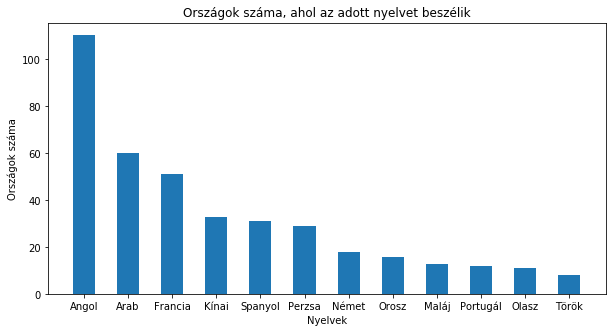
\includegraphics[width=150mm, keepaspectratio]{figures/languagesInCountries.png}
\caption{Országok száma, melyekben az adott nyelvet beszélik. \cite{nyelvekvilaga}}
\end{figure}

Számos nyelvet beszélnek világszerte az angol mellett, sokak számára viszont az angol nem az anyanyelvük, estleg egyáltalán nem beszélik azt. Beszédfelismerés során tehát szükséges egyéb hivatalos nyelveket is vizsgálni és kutatni.

Az orosz több mint 140 millió ember anyanyelve és további 110 millióan használják az oroszt második nyelvként\footnote{Az orosz nyelv, Wikipedia \url{https://hu.wikipedia.org/wiki/Orosz_nyelv}}, így az orosz nyelv igen fontos szerepet tölt be a nemzetközi porondon. Az 1.1-es ábrán látható, hogy elterjedt nyelvnek számít több országban is. Az end-to-end technológia és a neurális hálók által nyújtott lehetőségek megkönnyítik a nyelvek közti átállást, így egy angoltól eltérő nyelv vizsgálata és kutatása gördülékenyen megvalósítható egy angol nyelvű példa alapján.

Munkám az orosz nyelvű beszédfelismerés lehetőségeit mutatja-be, de segítségével tetszőleges idegen nyelven, az itt bemutatott irányelvek mentén, lehetséges a beszédfelismerés kutatása és pontosítása.

\section{Diplomaterv felépítése}

A követelmények elemzése fejezetben a munkám főbb szempontjai, a sarkalatos pontok és kikötések kerülnek részletezésre, kifejtésre. Ezen pontok kidolgozásának módjai, esetleges nehézségei kerülnek említésre. Felsorakoztatom a tervezés előtt felmerült ötleteket, azok megvalósításának lehetőségeit.

Az elméleti összefoglaló rész a beszédfelismerés teóriájával foglalkozik, különösképp kitérve a neurális hálókat alkalmazó implementációra és azok alapjaira. Továbbá tartalmazza az eddigi legjobb megoldásokat, melyeket össze is hasonlít, röviden értékelve azok sikerességét. A levonható következtetések fényében felvázolja a fejlesztés kiindulási alapjának tekinthető állapotot és tervezésbeli döntéseket.

A tervezés és fejeztet magába foglalja az előzetes döntéseket, a lehetséges kísérletek várható eredményét. A döntési lehetőségeket, értékelve és az azok mögötti ötleteket, esetleges alternatívákkal kiegészítve.

Az implementáció fejezetben a választott megoldások megvalósítását írom le, alátámasztva és indokolva azok sikerességét.

Az összefoglaló tartalmazza az elért eredmények bemutatását, azok értékelését és a végső következtetések levonását, illetve a további kutatási lehetőségek felvázolását.